\documentclass[conference]{IEEEtran}
\IEEEoverridecommandlockouts
\usepackage{cite}
\usepackage{amsmath,amssymb,amsfonts}
\usepackage{graphicx}
\usepackage{booktabs}
\usepackage{enumitem}
\usepackage{tikz}
\usetikzlibrary{arrows.meta,positioning}

\newcommand{\sat}{\operatorname{sat}}
\newcommand{\sign}{\operatorname{sign}}
\newcommand{\diag}{\operatorname{diag}}
\newcommand{\skewm}[1]{[#1]_\times}

\begin{document}

\title{Static-Mount Quadrotor Attitude Testbed:\\ Hardware Physics, Identification, Modelling, and the Complete Controller Suite\\
{\footnotesize Mathematical foundations for offline simulation, digital-twin, and hardware execution}}

\author{\IEEEauthorblockN{Gandhi Contreras}
\IEEEauthorblockA{\textit{Electrical and Computer Engineering}, New Mexico State University, Las Cruces, NM, USA \\ gandhico@nmsu.edu}}

\maketitle

\begin{abstract}
This paper develops the mathematics of a quadrotor rigidly mounted at its centre of mass on a low-friction pivot, so that translation is constrained and the three rotational degrees of freedom remain --- the safe configuration in which full attitude control authority is exercised before free flight. The treatment is physics-complete: the LiPo energy source and its sag model, electronic speed controllers and brushless motor electromechanics, propeller thrust/reaction aerodynamics and rotor gyroscopic effects, the mixer that maps rotor commands to body wrench, MEMS inertial sensing and attitude estimation, and the sampled control loop. Rigid-body attitude dynamics are derived in both quaternion and Euler parameterizations; the identification of inertia, thrust, and drag-torque coefficients is formulated as static and dynamic experiments linear in the parameters; and the complete controller suite is developed: quaternion PD/PID with bandwidth-based gain design, LQR and LQG on the attitude linearization, backstepping on the rotation group, sliding-mode control, and nonlinear model predictive control, together with the mixer allocation and its saturation handling.
\end{abstract}

\begin{IEEEkeywords}
Quadrotor, attitude dynamics, quaternion control, BLDC, ESC, mixer allocation, LQR, LQG, backstepping, SMC, NMPC.
\end{IEEEkeywords}

%====================================================================
\section{Introduction}
Mounting a quadrotor at its centre of mass on a 3-DOF pivot removes translation while preserving the exact rotational dynamics, actuators, sensing, and software of free flight; it is the standard bridge between simulation and flight. The state is attitude and body rate,
\begin{equation}
x = (q,\ \omega),\qquad q\in\mathbb S^3\subset\mathbb R^4,\ \ \omega\in\mathbb R^3,
\end{equation}
with unit quaternion $q = [q_0,\ q_v^{\!\top}]^{\!\top}$ (scalar first) and $\omega$ the body angular velocity. Inputs are the four rotor thrust commands $u = [u_1,\dots,u_4]^{\!\top}$. Our controller conventions and gains follow the quaternion PD architecture validated in our simulation campaigns (Skydio-X2- and Crazyflie-2-class parameters).

%====================================================================
\section{Hardware Physics: Battery to Body Torque}

\begin{figure*}[!t]
\centering
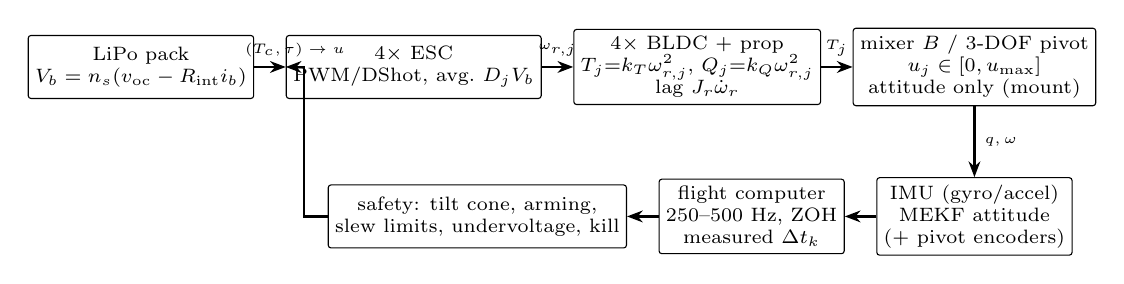
\begin{tikzpicture}[
  node distance=3mm and 4mm,
  blk/.style={draw, rounded corners=1pt, align=center, font=\scriptsize, inner sep=2.5pt, minimum height=8mm},
  lbl/.style={font=\tiny, align=center},
  arr/.style={-{Stealth[length=2mm]}, thick}
]

\node[blk] (bat) {LiPo pack\\ $V_b = n_s(v_{\mathrm{oc}} - R_{\mathrm{int}}i_b)$};
\node[blk, right=of bat] (esc) {$4\times$ ESC\\ PWM/DShot, avg.\ $D_jV_b$};
\node[blk, right=of esc] (rot) {$4\times$ BLDC + prop\\ $T_j{=}k_T\omega_{r,j}^2$, $Q_j{=}k_Q\omega_{r,j}^2$\\ lag $J_r\dot\omega_r$};
\node[blk, right=of rot] (mix) {mixer $B$ / 3-DOF pivot\\ $u_j\in[0,u_{\max}]$\\ attitude only (mount)};
\node[blk, below=9mm of mix] (sens) {IMU (gyro/accel)\\ MEKF attitude\\ (+ pivot encoders)};
\node[blk, left=of sens] (fc) {flight computer\\ 250--500 Hz, ZOH\\ measured $\Delta t_k$};
\node[blk, left=of fc] (safe) {safety: tilt cone, arming,\\ slew limits, undervoltage, kill};
\draw[arr] (bat) -- (esc);
\draw[arr] (esc) -- node[lbl, above] {$\omega_{r,j}$} (rot);
\draw[arr] (rot) -- node[lbl, above] {$T_j$} (mix);
\draw[arr] (mix) -- node[lbl, right] {$q,\omega$} (sens);
\draw[arr] (sens) -- (fc);
\draw[arr] (fc) -- (safe);
\draw[arr] (safe.west) -- ++(-3mm,0) |- node[lbl, pos=0.75, above] {$(T_c,\tau)\to u$} (esc.west);
\end{tikzpicture}
\caption{Static-mount quadrotor signal chain: battery sag scales all thrusts; the mixer's non-negativity clip is the allocation constraint; the mount removes translation while preserving the attitude loop.}
\label{fig:chain}
\end{figure*}
\subsection{Energy source}
A lithium-polymer pack of $n_s$ cells supplies $V_b = n_s\,v_{\mathrm{cell}}(\mathrm{SoC}, i_b)$ with the loaded cell voltage modelled as
\begin{equation}
v_{\mathrm{cell}} = v_{\mathrm{oc}}(\mathrm{SoC}) - R_{\mathrm{int}}\, i_b ,
\end{equation}
open-circuit voltage falling from $\sim$4.2 to $\sim$3.3~V/cell over discharge and internal resistance $R_{\mathrm{int}}$ producing sag under thrust transients. Because rotor thrust at fixed duty scales with $V_b^2$ through the speed map below, \emph{battery state enters the control loop as an input-gain disturbance}; hover-throttle drift over a run is the visible symptom, and gain scheduling on measured $V_b$ is the standard compensation. Peak current is bounded by the pack C-rating; undervoltage lockout is a safety event.

\subsection{ESC and brushless motor}
Each electronic speed controller synthesizes three-phase excitation (six-step or field-oriented) from the DC bus at duty $D_j\in[0,1]$. Averaged over the commutation period, the motor obeys the DC-equivalent model
\begin{equation}
L_a\dot i_j + R_m i_j + k_e\,\omega_{r,j} = D_j V_b,\qquad
\tau_{m,j} = k_t\, i_j ,
\end{equation}
and the rotor speed dynamics
\begin{equation}
J_r\,\dot\omega_{r,j} = \tau_{m,j} - k_Q\,\omega_{r,j}^2 - b_r\,\omega_{r,j},
\label{eq:rotorspeed}
\end{equation}
a first-order lag (time constant typically 20--80~ms) between command and thrust that must be included whenever the attitude bandwidth approaches it.

\subsection{Propeller aerodynamics and rotor moments}
Momentum/blade-element theory gives the quasi-static maps
\begin{equation}
T_j = k_T\,\omega_{r,j}^2,\qquad Q_j = k_Q\,\omega_{r,j}^2,
\end{equation}
thrust along the body $z$ axis and aerodynamic drag torque about it, with signs alternating by rotor handedness. Two additional rotor-physics torques act on the body: the \emph{gyroscopic} moment of the spinning rotors under body rotation,
\begin{equation}
\tau_{\mathrm{gyro}} = -\sum_j J_r\,\omega_{r,j}\ (\omega \times \hat z_b)\,\sigma_j,
\qquad \sigma_j = \pm1,
\end{equation}
and the \emph{inertial reaction} $-J_r\dot\omega_{r,j}\hat z_b\sigma_j$ during rotor accelerations --- both small for matched rotor pairs but included in the refined model.

\subsection{Mixer (control allocation)}
With rotor positions $(x_j, y_j)$ in the body frame and yaw coefficients $\kappa_j = \pm k_Q/k_T$, the rotor thrusts map to collective thrust and body torques by
\begin{equation}
\begin{bmatrix} T\\ \tau_x\\ \tau_y\\ \tau_z\end{bmatrix}
= B\,u,\qquad
B = \begin{bmatrix}
1&1&1&1\\
y_1&y_2&y_3&y_4\\
-x_1&-x_2&-x_3&-x_4\\
\kappa_1&\kappa_2&\kappa_3&\kappa_4
\end{bmatrix},
\label{eq:mixer}
\end{equation}
inverted as $u = B^{-1}[T_c,\ \tau^{\!\top}]^{\!\top}$ followed by the physical clip $u_j\in[0,\,u_{\max}]$ --- the non-negativity of thrust is the essential allocation constraint: torque authority shrinks as collective approaches either limit. On the static mount $T_c$ is a free parameter (typically near hover-equivalent) chosen to centre the rotors in their linear range. Representative X2-class values from our campaign: arms $(\pm0.14,\ \pm0.18)$~m, $\kappa = \mp0.0201$, $u_{\max} = 13$~N per rotor.

\subsection{Sensing and the loop}
Attitude is sensed by a MEMS IMU: gyroscope $\omega_m = \omega + b_g + \eta_g$ (bias random walk $\dot b_g = \eta_b$) and accelerometer, fused by a complementary/Mahony filter or multiplicative EKF; on instrumented mounts, pivot encoders provide ground-truth Euler angles with quantization $2\pi/N_{\mathrm{enc}}$. The control loop runs at $f_s$ (250--500~Hz class) with ZOH outputs to the ESCs (PWM/DShot), realized-period jitter, and the measured-$\Delta t$ rule for all discrete updates. Safety envelope: attitude cone limit on the mount, rotor arming logic, command slew limits, battery undervoltage and ESC/motor thermal derating, and kill switch forcing $u = 0$.

%====================================================================
\section{Attitude Dynamics}
\subsection{Kinematics}
Unit-quaternion kinematics (scalar-first, body rates):
\begin{equation}
\dot q = \tfrac12\, q \otimes \begin{bmatrix}0\\ \omega\end{bmatrix}
= \tfrac12\,\Omega(\omega)\,q,
\end{equation}
with $\otimes$ the Hamilton product; the rotation matrix is $R(q) = I + 2q_0\skewm{q_v} + 2\skewm{q_v}^2$. Euler ZYX angles $(\phi,\theta,\psi)$ relate by the standard kinematic map $\dot\Theta = W(\Theta)\,\omega$, singular at $\theta = \pm\pi/2$ --- the reason the quaternion form is primary.

\subsection{Euler's equations on the mount}
With inertia $I_B = \diag(I_{xx}, I_{yy}, I_{zz})$ about the pivot (equal to the c.o.m. inertia for a centred mount),
\begin{equation}
I_B\,\dot\omega = -\,\omega\times I_B\,\omega + \tau + \tau_{\mathrm{gyro}} + \tau_{f} + \tau_{g},
\label{eq:euler}
\end{equation}
where $\tau$ is the mixer torque of \eqref{eq:mixer}, $\tau_f = -B_f\omega - \tau_c\tanh(\omega/\epsilon)$ the pivot friction, and $\tau_g = m\,r_{\mathrm{cg}}\times R^{\!\top}g e_3$ the gravitational torque of any centre-of-mass offset $r_{\mathrm{cg}}$ from the pivot (zero for a perfectly centred mount; identified in practice). Equations \eqref{eq:euler} with the rotor lag \eqref{eq:rotorspeed} constitute the full nonlinear model.

\subsection{Attitude error and linearization}
For a reference $q_r$, the error quaternion and its vector part are
\begin{equation}
q_e = q_r \otimes q^{*},\qquad e_q = \sign(q_{e,0})\,q_{e,v},
\label{eq:qerr}
\end{equation}
the sign enforcing shortest-path correction (the double cover of $\mathrm{SO}(3)$). For small errors $q_e \approx [1,\ \tfrac12\delta\Theta^{\!\top}]^{\!\top}$, and \eqref{eq:euler} linearizes per axis to
\begin{equation}
I_{ii}\,\ddot{\delta\Theta}_i + B_{f,ii}\,\dot{\delta\Theta}_i = \tau_i,
\end{equation}
three decoupled double integrators with damping --- the design plant for the linear controllers, assembled as $\dot x = Ax + B\tau$ with $x = [\delta\Theta^{\!\top},\ \omega^{\!\top}]^{\!\top}\in\mathbb R^6$.

%====================================================================
\section{Identification}

\begin{figure}[!t]
\centering
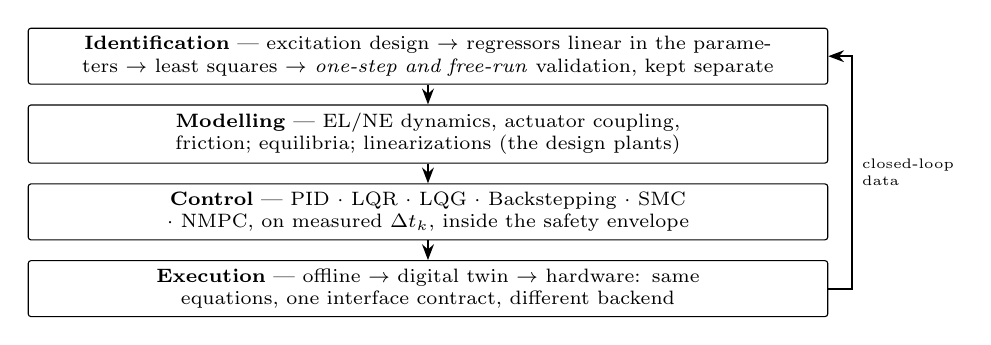
\begin{tikzpicture}[
  node distance=2.5mm,
  blk/.style={draw, rounded corners=1pt, align=center, font=\scriptsize, inner sep=3pt, text width=0.82\columnwidth},
  arr/.style={-{Stealth[length=2mm]}, thick}
]
\node[blk] (id) {\textbf{Identification} --- excitation design $\to$ regressors linear in the parameters $\to$ least squares $\to$ \emph{one-step and free-run} validation, kept separate};
\node[blk, below=of id] (mod) {\textbf{Modelling} --- EL/NE dynamics, actuator coupling, friction; equilibria; linearizations (the design plants)};
\node[blk, below=of mod] (ctl) {\textbf{Control} --- PID $\cdot$ LQR $\cdot$ LQG $\cdot$ Backstepping $\cdot$ SMC $\cdot$ NMPC, on measured $\Delta t_k$, inside the safety envelope};
\node[blk, below=of ctl] (exe) {\textbf{Execution} --- offline $\to$ digital twin $\to$ hardware: same equations, one interface contract, different backend};
\draw[arr] (id) -- (mod);
\draw[arr] (mod) -- (ctl);
\draw[arr] (ctl) -- (exe);
\draw[arr] (exe.east) -- ++(3mm,0) |- node[font=\tiny, pos=0.25, right, align=left] {closed-loop\\ data} (id.east);
\end{tikzpicture}
\caption{The workflow every platform in this series follows: identification feeds modelling, modelling feeds the controller suite, and all stages run unchanged across the three execution targets; closed-loop records return to identification.}
\label{fig:workflow}
\end{figure}
\begin{enumerate}[label=E\arabic*)]
\item \emph{Thrust and drag maps (static)}: on a thrust stand or via the mount's load path, sweep $D_j$ and record $\omega_r$ (ESC telemetry), thrust and torque: least squares on $T = k_T\omega_r^2$, $Q = k_Q\omega_r^2$ (linear in $k_T,k_Q$); repeat across battery voltages to expose the $V_b$ gain dependence.
\item \emph{Rotor lag}: step the command, fit the first-order response of \eqref{eq:rotorspeed} linearized about the operating speed.
\item \emph{Inertia}: (a) bifilar/compound-pendulum swings of the airframe about each axis, $I = \kappa_g/\omega_n^2$ from measured periods; (b) on-mount dynamic identification --- apply torque doublets through the mixer and regress \eqref{eq:euler}, which is linear in $(I_{xx},I_{yy},I_{zz}, B_f, \tau_c, m r_{\mathrm{cg}})$ given reconstructed $\dot\omega$ (filtered differentiation of gyro rates).
\item \emph{Black-box cross-check}: per-axis ARX on doublet/PRBS records; validation reported as one-step and free-run fits separately, on held-out data.
\end{enumerate}

%====================================================================
\section{Control Suite}
All laws command the wrench $(T_c, \tau)$, allocate through \eqref{eq:mixer} with clipping, use gyro rates directly (bias-corrected) and filtered derivatives elsewhere, and advance with measured $\Delta t_k$.

\subsection{Quaternion PD/PID (implemented baseline)}
\begin{equation}
\tau = -K_q\,e_q - K_\omega\,\omega + K_i\!\int e_q\,dt,
\label{eq:qpd}
\end{equation}
with $e_q$ from \eqref{eq:qerr}, integral term optional (with conditional anti-windup) since the mount has no steady disturbance torque beyond $\tau_g$. Bandwidth-based gain design used in our campaigns:
\begin{equation}
K_q = 2\,I_B\,\omega_n^2,\qquad K_\omega = 2\,\zeta\,\omega_n\, I_B,
\end{equation}
elementwise with $\omega_n = [4,\ 4,\ 3.5]$~rad/s, $\zeta = 0.95$ (validated values), then $\tau$ clipped to the allocation-feasible set. Nominal closed loop per axis: $\ddot{\delta\Theta} + 2\zeta\omega_n\dot{\delta\Theta} + \omega_n^2\,\delta\Theta = 0$.

\subsection{LQR and LQG}
On the six-state linearization, $\tau = -K_{\mathrm{lqr}}x$ with $K_{\mathrm{lqr}}$ from the CARE $(A,B,Q,R)$; Bryson scaling on angle/rate/torque bounds initializes $(Q,R)$. LQG replaces $x$ by the estimate of a Kalman--Bucy filter driven by the fused attitude and gyro measurements; with IMU-only sensing the filter is the attitude MEKF whose error-state covariance supplies $L$; separation holds nominally, and the estimator propagates with measured $\Delta t_k$.

\subsection{Backstepping on the rotation group}
Two-step design with $z_1 = e_q$ and desired rate $\omega_d = -c_1 z_1$: define $z_2 = \omega - \omega_d$. Using $\dot e_q \approx \tfrac12(q_{e,0} I + \skewm{q_{e,v}})\,z_2 - \tfrac12 c_1 (\cdot)z_1$ and the Lyapunov function
\begin{equation}
V = 2\,(1 - |q_{e,0}|) + \tfrac12\, z_2^{\!\top} I_B\, z_2 ,
\end{equation}
the control
\begin{equation}
\tau = \omega\times I_B\omega - I_B\bigl(c_2 z_2 + \tfrac12 z_1\bigr) + I_B\,\dot\omega_d
\end{equation}
yields $\dot V \le -c_1\,\kappa\,\|z_1\|^2 - c_2\,\lambda_{\min}(I_B)\|z_2\|^2$ in the shortest-path half-cover, giving almost-global asymptotic stability (the antipodal equilibrium is the unavoidable topological obstruction).

\subsection{Sliding-mode control}
Per-axis surfaces on the error state, $s = \omega + \Lambda\,e_q$ ($\Lambda\succ0$ diagonal), control
\begin{equation}
\tau = \omega\times I_B\omega - I_B\Lambda\,\dot e_q^{\,\mathrm{nom}} - K_s\,\sat(s/\phi),
\end{equation}
with $K_s$ exceeding the matched uncertainty bound (rotor-map error, $\tau_g$ misidentification); boundary layer $\phi$ sets the chatter/accuracy trade, and reaching is certified by $\tfrac{d}{dt}\tfrac12 s^{\!\top}I_B s \le -\sum_i(K_{s,i} - \bar\rho_i)|s_i|$.

\subsection{NMPC}
Receding-horizon OCP on the full model \eqref{eq:euler} (quaternion state, RK4 discretization at $\Delta t_p$):
\begin{align}
\min_{\{u_k\}}\ &\sum_{k=0}^{N-1}\Bigl( \|e_{q,k}\|_Q^2 + \|\omega_k\|_{Q_\omega}^2 + \|u_k - u_h\|_R^2 \Bigr) + V_f(x_N)\nonumber\\
\text{s.t. }\ & 0 \le u_{j,k} \le u_{\max},\quad \text{attitude cone } \|e_{q,k}\|\le\bar e,
\end{align}
with $u_h$ the hover-equivalent rotor set and $V_f$ the LQR terminal cost. Real-time reductions proven on our other platforms apply unchanged: short horizon, move blocking, warm start, and candidate-grid search centred on the allocation of the backstepping/PD wrench. Rotor non-negativity makes allocation-aware NMPC strictly stronger than post-hoc clipping near the thrust limits --- the regime where it earns its cost.

%====================================================================
\section{Execution Modes and Conclusion}
Offline simulation integrates \eqref{eq:rotorspeed}--\eqref{eq:euler} with sensor and battery models injectable; the digital twin exposes the same wrench/attitude contract in the vendor virtual environment; hardware is the mounted vehicle with the safety envelope (attitude cone, arming, slew, undervoltage, kill). The controller mathematics above are common to all three. The static mount thereby delivers what it promises: the complete attitude-control mathematics of the free-flying vehicle --- energy source to body torque, identification to NMPC --- exercised under laboratory constraint, so that the transition to free flight changes only the outer translational loops, not the foundations.

\bibliographystyle{IEEEtran}
\begin{thebibliography}{9}
\bibitem{mahony2012} R.~Mahony, V.~Kumar, and P.~Corke, ``Multirotor aerial vehicles: Modeling, estimation, and control of quadrotor,'' \emph{IEEE Robot. Autom. Mag.}, vol.~19, no.~3, pp. 20--32, 2012.
\bibitem{leishman2006} J.~G. Leishman, \emph{Principles of Helicopter Aerodynamics}, 2nd ed. Cambridge Univ. Press, 2006.
\bibitem{markley2014} F.~L. Markley and J.~L. Crassidis, \emph{Fundamentals of Spacecraft Attitude Determination and Control}. Springer, 2014.
\bibitem{khalil2002} H.~K. Khalil, \emph{Nonlinear Systems}, 3rd ed. Prentice Hall, 2002.
\bibitem{krstic1995} M.~Krsti\'c, I.~Kanellakopoulos, and P.~Kokotovi\'c, \emph{Nonlinear and Adaptive Control Design}. Wiley, 1995.
\bibitem{utkin1992} V.~Utkin, \emph{Sliding Modes in Control and Optimization}. Springer, 1992.
\bibitem{rawlings2017} J.~B. Rawlings, D.~Q. Mayne, and M.~Diehl, \emph{Model Predictive Control}, 2nd ed. Nob Hill, 2017.
\bibitem{ljung1999} L.~Ljung, \emph{System Identification: Theory for the User}, 2nd ed. Prentice Hall, 1999.
\end{thebibliography}

\end{document}
